\documentclass[AMS,STIX2COL]{WileyNJD-v2}

\usepackage{amsthm,amsmath,natbib,tabularx,graphicx,hyperref}

\authormark{Goode, Ries, and McClernon. \emph{Characterizing climate pathways using feature importance on echo state networks}}

% for commenting
\newcommand{\dr}[1]{\textcolor{blue}{DR: #1}}
\newcommand{\kg}[1]{\textcolor{orange}{KG: #1}}
\newcommand{\km}[1]{\textcolor{green}{KM: #1}}
\newcommand{\add}[1]{\textcolor{purple}{#1}}

% add S in front of sections, figures, and tables
\renewcommand{\thesection}{S.\arabic{section}}
\renewcommand{\thesubsection}{\thesection.\arabic{subsection}}
\renewcommand{\thefigure}{S\arabic{figure}}
\renewcommand{\thetable}{S\arabic{table}}

\DeclareCaptionLabelSeparator{mycolon}{\hspace{0.1cm}}
\captionsetup[figure]{labelsep=mycolon}
\captionsetup[table]{labelsep=mycolon}

\begin{document}

\begin{center}
{\Large \textbf{Supplemental Material}}
\end{center}

This document contains additional results from the simulations study and the Mount Pinatubo eruption example associated with the article \emph{Characterizing climate pathways using feature importance on echo state networks}.

\section{Simulation Study Additional Results}

The remainder of the simulation study results are described below. These results include a comparison of feature importance for all variance values ($\sigma_z$, $\sigma_\delta$, and $\sigma_\epsilon$) and an analysis of the effect of the parameters $\rho_z$, $\rho_\delta$, $\phi_z$, and $\phi_\delta$ on the feature importance.

Figure \ref{fig:pfi-supplement} shows stPFI for variables ${\bf Z}_1$ and ${\bf Z}_2$, while varying $\sigma_z,\sigma_{\delta},\sigma_{\epsilon}$ and number of blocks. stPFI tends to be more pronounced with an increase in the block size, as well as smoother. stPFI does pick up on importance for ${\bf Z}_1$ even though ${\bf Z}_1$ has no direct impact on the response, and worse, this effect grows with increasing block size. An increase in the variation of $\sigma_z$ corresponds with a flattening of stPFI across the board which is not surprising since the true importance is being masked by noise. The random effect variability $\sigma_{\delta}$ and white noise variability $\sigma_{\epsilon}$ do not have a large impact on stPFI, but  increases of $\sigma_z$ do reduce the FI values in magnitude and in the range of when stPFI picks up the importance.  Regardless of the standard deviations being increased by an order of magnitude, stPFI still has a clear signal.

Figure \ref{fig:zfi-supplement} shows stZFI for variables ${\bf Z}_1$ and ${\bf Z}_2$, while varying $\sigma_z,\sigma_{\delta},\sigma_{\epsilon}$ and number of blocks. stZFI tends to be more pronounced with an increase in the block size, as well as more smooth. In some situations, stZFI does pick up on importance for ${\bf Z}_1$ even though ${\bf Z}_1$ has no direct impact on the response. However, this effect is much smaller in magnitude compared to the true importance of variable ${\bf Z}_2$. An increase in the variation of $\sigma_z$ corresponds with a flattening of stZFI across the board, as well as less smooth FI, which is not surprising since the true importance is being masked by noise. The random effect variability $\sigma_{\delta}$ and white noise variability $\sigma_{\epsilon}$ do not have a large impact on stZFI, but  increases of $\sigma_z$ do reduce the FI values in magnitude and in the range of when stZFI picks up the importance. Regardless of the standard deviations being increased by an order of magnitude, stZFI still has a clear signal.

Figure \ref{fig:pfi-supplement-rhophi} shows stPFI for variables ${\bf Z}_1$ and ${\bf Z}_2$, while varying $\rho_z,\rho_{\delta},\phi_z,\phi_{\delta}$ with a block size of 3. We restricted block size to 3 for brevity, because there did not appear to be any interaction between block size and these parameters. The main difference is when $\rho_z$ is smaller, stPFI is relatively larger for ${\bf Z}_1$ and relatively smaller for ${\bf Z}_2$ compared to when $\rho_z$ is large, meaning the performance of stPFI is better with larger $\rho_z$. Larger autocorrelation of the random effect, $\rho_{\delta}$, appears to make stPFI perform worse (relatively larger stPFI for ${\bf Z}_1$ and relatively smaller stPFI for ${\bf Z}_2$). The spatial range parameters, $\phi_z,\phi_{\delta}$ appear to have minimal impact on stPFI.

Figure \ref{fig:zfi-supplement-rhophi} shows stZFI for variables ${\bf Z}_1$ and ${\bf Z}_2$, while varying $\rho_z,\rho_{\delta},\phi_z,\phi_{\delta}$ with a block size of 3. We restricted block size to 3 for brevity because there did not appear to be any interaction between block size and these parameters. The main difference is when $\rho_z$ is smaller, stZFI is relatively smaller for ${\bf Z}_2$ compared to when $\rho_z$ is large, meaning the performance of stZFI is better with larger $\rho_z$. Larger autocorrelation of the random effect, $\rho_{\delta}$, appears to make stZFI perform slightly worse (relatively smaller stZFI for ${\bf Z}_2$), but this effect appears small. The spatial range parameters, $\phi_z,\phi_{\delta}$ appear to have minimal impact on stZFI.

\section{Mount Pinatubo Application Additional Results}

Recall that the ESNs in the main text for capturing the relationships between AOD and stratospheric temperature are trained on MERRA-2 data from 1980-1995. The model inputs of lagged values of AOD and stratospheric temperature are used to forecast stratospheric temperature one month in the future. The following subsections contain information on how the hyperparameters are selected, additional results from the model validation, and additional feature importance results. Note that all models considered in the following analyses have the same embedding vector values of $m=5$ and $\tau^*=1$.

\subsection{Hyperparameter Selection}

The hyperparameters for the ESNs in the main text are selected by considering a grid of parameter values and determining the set of values that return the best predictive performance on a held out set of data. In particular, the data are split into training and testing sets by the year divisions of 1980-1993 and 1994-1995, respectively. The predictive performance is assessed using weighted root mean square error (RMSE) where the weights are assigned using cosine latitude as described in the main text.

The hyperparameters included in the grid are the number of hidden units ($n_h$), the scaling memory parameter ($\nu$), the uniform distribution widths for generating $\textbf{U}$ and $\textbf{W}$ ($a_u$ and $a_w$, respectively), the Bernoulli parameters used for generating $\textbf{U}$ and $\textbf{W}$ ($\pi_u$ and $\pi_w$, respectively), and the ridge regression penalty parameter ($\lambda_r$). The values considered for each of these parameters are listed in Table \ref{tab:hps}. In addition to considering all combinations of these parameter values, each set of hyperparameters is used to train an ESN with and without a quadratic term in the ridge regression.

\begin{table}[]
    \centering
    \begin{tabular}{cl}
    \hline
    Parameter & Values \\
    \hline
    $n_h$ & 50, 100, 500, 1000, 2000\\
    $\nu$ & 0, 0.2, 0.4, 0.6, 0.8, 1\\
    $a_u$ & 0.1, 0.5, 1\\
    $a_w$ & 0.1, 0.5, 1\\
    $\pi_u$ & 0.1, 0.5, 0.9\\
    $\pi_w$ & 0.1, 0.5, 0.9\\
    $\lambda_r$ & 0.1, 5, 20, 50, 100, 500\\
    Quadratic Term & Yes, No\\
    \hline
    \end{tabular}
    \caption{ESN hyperparameters and corresponding values considered in the hyperparameter tuning grid search.}
    \label{tab:hps}
\end{table}

The other adjustable value that we consider in the grid search is the number of principal components included. The models in the main text use the first five principal components from both AOD and stratospheric temperature. For the hyperparameter tuning, the full grid search is implemented for both the first five and ten principal components. Note that the percent of variability captured by the first five and ten principal components for AOD are 59.9\% and 85.6\%, respectively. The proportion of variability captured by the first five and ten principal components for stratospheric temperature are 76.5\% and 88.8\%, respectively.

In total, 58,320 ($=5\times6\times3\times3\times3\times3\times6\times2\times2$) ESN architectures are considered. For each architecture, five ESNs are trained to account for the random variability in the $\textbf{U}$ and $\textbf{W}$ matrices. For each model, a weighted RMSE is computed that includes all locations and times in the test data. A single assessment metric is then obtained for each ESN architecture by computing an average of the weighted RMSEs from the five replicates of an architecture. The same process is taken to obtain an averaged weighted RMSE on the training data for each model architecture considered.

Table \ref{tab:hp_top} contains the twenty five sets of hyperparameters that resulted in the lowest test data averaged weighted RMSEs. For simplicity, we will refer to `averaged weighted RMSE' as `RMSE' for the remainder of this subsection. The top nine sets of hyperparameter values have the same RMSE out to at least six digits. These sets all have the same number of principal components (5), number of hidden units (1000), uniform distribution width for $\textbf{U}$ (0.1), Bernoulli parameter for $\textbf{U}$ (0.1), memory scaling parameter (0), ridge regression parameter (5), and a quadratic term in the ridge regression. The other parameters appear to have no effect on the test RMSE (at least to 6 digits). The RMSEs are also the same out to 6 digits within parameter sets 10-18. Note that the difference from parameter sets 1-9 to 10-18 is the removal of the quadratic term in the ridge regression. Parameter sets 19-25 return to having a quadratic term, but the parameter $\nu$ changes to 0.2. 

Note that $\nu=0$ cancels out the term in the hidden state of the ESN containing $\textbf{W}$. By removing this term, the recursive aspect of the ESN is removed. When selecting the hyperparameters to use in the final ESN for analysis, we opt to use the parameter values in row 19 instead of row 1. We want the model to include the recursive element, and there is only a minimal increase in the test RMSE from 0.822802 to 0.824966.

\begin{table*}[ht]
\centering
%\begin{tabularx}{\textwidth}{ccccccccccc}
\begin{tabular}{ccccccccccc}
\hline
Order & No. PCs & $n_h$ & $a_u$ & $a_w$ & $\pi_u$ & $\pi_w$ & $\nu$ & $\lambda_r$ & Quadratic Term & RMSE \\
\hline
1 & 5 & 1000 & 0.1 & 0.1 & 0.1 & 0.1 & 0 & 5 & Yes & 0.822802 \\ 
2 & 5 & 1000 & 0.1 & 0.5 & 0.1 & 0.1 & 0 & 5 & Yes & 0.822802 \\ 
3 & 5 & 1000 & 0.1 & 1 & 0.1 & 0.1 & 0 & 5 & Yes & 0.822802 \\ 
4 & 5 & 1000 & 0.1 & 0.1 & 0.1 & 0.5 & 0 & 5 & Yes & 0.822802 \\ 
5 & 5 & 1000 & 0.1 & 0.5 & 0.1 & 0.5 & 0 & 5 & Yes & 0.822802 \\ 
6 & 5 & 1000 & 0.1 & 1 & 0.1 & 0.5 & 0 & 5 & Yes & 0.822802 \\ 
7 & 5 & 1000 & 0.1 & 0.1 & 0.1 & 0.9 & 0 & 5 & Yes & 0.822802 \\ 
8 & 5 & 1000 & 0.1 & 0.5 & 0.1 & 0.9 & 0 & 5 & Yes & 0.822802 \\ 
9 & 5 & 1000 & 0.1 & 1 & 0.1 & 0.9 & 0 & 5 & Yes & 0.822802 \\ 
10 & 5 & 1000 & 0.1 & 0.1 & 0.1 & 0.1 & 0 & 5 & No & 0.823666 \\ 
11 & 5 & 1000 & 0.1 & 0.5 & 0.1 & 0.1 & 0 & 5 & No & 0.823666 \\ 
12 & 5 & 1000 & 0.1 & 1 & 0.1 & 0.1 & 0 & 5 & No & 0.823666 \\ 
13 & 5 & 1000 & 0.1 & 0.1 & 0.1 & 0.5 & 0 & 5 & No & 0.823666 \\ 
14 & 5 & 1000 & 0.1 & 0.5 & 0.1 & 0.5 & 0 & 5 & No & 0.823666 \\ 
15 & 5 & 1000 & 0.1 & 1 & 0.1 & 0.5 & 0 & 5 & No & 0.823666 \\ 
16 & 5 & 1000 & 0.1 & 0.1 & 0.1 & 0.9 & 0 & 5 & No & 0.823666 \\ 
17 & 5 & 1000 & 0.1 & 0.5 & 0.1 & 0.9 & 0 & 5 & No & 0.823666 \\ 
18 & 5 & 1000 & 0.1 & 1 & 0.1 & 0.9 & 0 & 5 & No & 0.823666 \\ 
19 & 5 & 1000 & 0.1 & 0.1 & 0.1 & 0.9 & 0.2 & 5 & Yes & 0.824477 \\
20 & 5 & 1000 & 0.1 & 0.5 & 0.1 & 0.9 & 0.2 & 5 & Yes & 0.824477 \\
21 & 5 & 1000 & 0.1 & 1 & 0.1 & 0.9 & 0.2 & 5 & Yes & 0.824477 \\ 
22 & 5 & 1000 & 0.1 & 0.1 & 0.1 & 0.5 & 0.2 & 5 & Yes & 0.824612 \\
23 & 5 & 1000 & 0.1 & 0.5 & 0.1 & 0.5 & 0.2 & 5 & Yes & 0.824612 \\
24 & 5 & 1000 & 0.1 & 1 & 0.1 & 0.5 & 0.2 & 5 & Yes & 0.824612 \\ 
25 & 5 & 1000 & 0.1 & 0.1 & 0.1 & 0.1 & 0.2 & 5 & Yes & 0.824966 \\
\hline
\end{tabular}
\caption{The sets of ESN hyperparameter values with the twenty five lowest test RMSEs.}
\label{tab:hp_top}
\end{table*}

Figure \ref{fig:hp_all} depicts the testing versus training RMSEs from all sets of hyperparameters considered.  The plot is repeated nine times, and the points in each repetition are colored by a different hyperparameter. The point colors are opaque, so a blending of colors indicates an overlap of points. The top left plot is colored by the number of principal components. There is a clear relationship with two different `U' shaped patterns resulting from the difference in the number of principal components. Models with five principal components result in the lowest test RMSEs, which led to our decision to work with five principal components for the final analysis. The other parameters that appear to have an effect on the generation of lower test RMSEs are $n_h$, $a_u$, $\nu$, and $\lambda_r$. $a_w$ and $\pi_w$ have minimal or no effect on the test RMSEs. $\pi_u$ and the quadratic term in the ridge regression have a small effect, but there is not a clear trend regarding a value that leads to the lowest test RMSEs. At least, if $\pi_u$ and the quadratic term affect the test RMSE, they are dependent on other hyperparameters.

Figure \ref{fig:hp_sub} again shows testing versus training RMSEs, but the results are subset to only include models with 5 principal components and test RMSEs less than 1. Furthermore, only plots of hyperparameters that have a clear effect on the test RMSE are included. This subsetting is done to better visualize the relationships bewteen the RMSEs and the hyperparameter values. We can see more clearly that lower test RMSEs tend to correspond to larger values of $n_h$, lower values of $a_w$, lower values of $\nu$, and middle range values of $\lambda_r$. As previously suspected, there is not a clear trend between lower test RMSEs and $\pi_u$ or an added quadratic term.

Figure \ref{fig:hp_uwidth} focuses on the relationship between $a_w$ and test RMSEs. Only results from ESNs fit with 5 principal components are included. The results are separated by the value of $n_h$, $a_w$ is plotted on the x-axis, and the points are colored by $\lambda_r$. Within each value of $n_h$, $a_w=0.1$ leads to the lowest test RMSEs. This visualization also highlights that the variability in test RMSEs within a value of $n_h$ tends to decrease as $a_w$ increases. This trend is most apparent as $n_h$ increases. Additionally, the value of $\lambda_r$ that leads to the lowest test RMSEs appears to be dependent on both $a_w$ and $n_h$.

Figure \ref{fig:hp_nu} considers the relationship bewteen $\nu$ and the test RMSE. We further focus on good performing hyperparameter sets by subsetting the RMSEs to only include 5 principal components and $a_w=0.1$ based on the results in Figure \ref{fig:hp_uwidth}. The results are separated by the value of $n_h$, the x-axis contains the value of $\nu$, and the points are colored by $\lambda_r$. Within all values of $n_h$, lower values of $\nu$ result in the lowest RMSEs, but there is a large amount of variability in RMSEs within a value of $\nu$ and $n_h$. Again, this visualization also shows the dependence between $\lambda_r$ and the lowest test RMSEs, but there is not a clear relationship between $\lambda_r$ and $\nu$ (within a value of $n_h$).

We further focus on better performing hyperparameter values in Figures \ref{fig:hp_nh_quad} and \ref{fig:hp_nh_upi} by only considering results from models fit with 5 principal components, $a_w=0.1$, and $\nu=0.2$. We elect to consider $\nu=0.2$ instead of $\nu=0$ here for the same reason we choose to use $\nu=0.2$ for our model analyzed in the main text. 

Figure \ref{fig:hp_nh_quad} highlights trends between $n_h$, $\lambda_r$, and the quadratic term. This plot shows that the quadratic term has an effect on the RMSE when $\lambda_r$ is small but only a minimal impact when $\lambda_r$ increases. This visualization also highlights the best performing set of hyperparameter values ($n_h$ of 1000 and $\lambda_r$ of 5), but there are other parameter sets that have similar performance including $n_h=2000$ and $\lambda_r=50$. Even a set of hyperparameters with a smaller values of $n_h$ (i.e., $n_h=50$ and $\lambda_r=0.1$) results in RMSEs that are within a range that could be considered not practically different.

Figure \ref{fig:hp_nh_upi} depicts the same values as Figure \ref{fig:hp_nh_quad}, but the points are colored by $\pi_u$. This figure shows that the best performing values of $\pi_u$ are dependent on the value of $\lambda_r$, and dependent on $n_h$ when $\lambda_r$ is small. For larger values of $\lambda_r$, larger values of $\pi_u$ result in smaller test RMSEs regardless of the value of $n_h$.

\subsection{Validation of ESN with Selected Hyperparameters} \label{sec:hps}

The results in this subsection are based on the final ESN architecture selected from the hyperparameter search.

Figure \ref{fig:merra2rmseanom} includes the results from all years of the time series block train/test split validation analysis. The message is similar to the figure in the main text that only included ESNs trained through even years: as the number of years in the training data increases, the test RMSEs stabilize and become more similar to the training RMSEs.

Figure \ref{fig:merra2rmse} contains results from the same analysis depicted in Figure \ref{fig:merra2rmseanom} except that the RMSEs are computed on the raw stratospheric temperature scale. Recall that the RMSEs in Figure \ref{fig:merra2rmseanom} are computed on the normalized anomalies of stratospheric temperature. This perspective shows that when the RMSEs are computed on the raw temperature scale seasonality appears to play a role in the predictive performance of the models. This is unsurprising since the model is trained with seasonality removed. Even though there appears to be more variability in the RMSEs over time on this scale, there is more stability in the test RMSEs when the models are trained over longer periods of time. The variability across ESNs within a time follows a similar pattern as seen in Figure \ref{fig:merra2rmseanom}.

Figure \ref{fig:merra2pred} shows predicted versus observed stratospheric temperatures on the raw temperature scale. Each plot is labeled by the year through which the model was trained on, leaving the remaining years through 1995 as testing data. For each of these plots, the predictions from one of the 25 ESNs with different $\textbf{U}$ and $\textbf{W}$ is randomly selected. It is easy to visually see the effect of model underfitting in the first plots where there is significant variation in the test sets. Models trying to forecast past 1990 without having seen Mount Pinatubo struggle. Models trained through Mount Pinatubo and its aftermath (1992 and beyond) are able to predict into the future well, even better than their training data. This is likely because the years following Pinatubo's eruption were less tumultuous. 

\subsection{Additional Feature Importance Results}

Figure \ref{fig:merra2blockave} shows FI computed with different block sizes from the ESNs trained with the final hyperparameter set selection. Each line represents the average FI computed over the 25 individual ensembles with different $\textbf{U}$ and $\textbf{W}$ matrices. The block size of six tends to have the largest FI magnitude, especially after the eruption events with stPFI. Since a larger block accounts for more time, it seem reasonable that it would lead to a larger FI magnitude. stZFI and stPFI clearly pick up the importance of AOD for forecasting stratospheric temperatures after both eruptions, regardless of block size.

Figure \ref{fig:merra2block} depicts the FIs from the individual ESNs, so it is possible to see the FI variability within a time. The variability across ESNs is most pronounced with stPFI, but the amount of FI variability is similar across block sizes within a FI type. Regardless of the FI variability due to the randomness in the ESN, clear FI trends are visible.

In order to assess the sensitivity of feature importance trends due to ESN hyperparameters. We computed FI from ESNs for two additional sets of hyperparameters that performed well based on the hyper parameter study in Section \ref{sec:hps}. The three sets of parameters are listed considered are listed in Table \ref{tab:hps3}. Note that Set 2 is the set used in the main text, and Sets 1 and 3 are the new additions. Note that the hyperparameters that vary are $n_h$, $\lambda_r$, and whether a quadratic term is included or not. Figures \ref{fig:hp_nh_quad} and \ref{fig:hp_nh_upi} highlight that the set of parameters with $n_h=2000$ has similar predictive performance as the set with $n_h=1000$. The set with $n_h=50$ has the largest test RMSE of these three sets but is chosen to include a case with a low number of hidden units. Again, 25 ESNs are trained for both sets of new hyperparameters with different random matrices of $\textbf{U}$ and $\textbf{W}$ in order to account for the sensitivity of the FI to these random matrices.

Figure \ref{fig:merra2fiparams} shows the FI results averaged over the 25 individual ESNs for the three sets of parameters, and Figure \ref{fig:merra2fiparamsvar} shows the FI results from the individual ESNs. The difference in FI magnitudes across parameter sets is more pronounced with stPFI than stZFI (especially for AOD). Interestingly, the FI for AOD computed with stPFI increases in magnitude as the number of hidden units decreases. For both stPFI and stZFI, the variability in FI across ESNs also increases as the the number of hidden units decreases.

\begin{table}[ht]
\centering
\begin{tabular}{rccc}
\hline
Hyperparameter & Set 1 & Set 2 & Set 3\\
\hline
No. PCs & 5 & 5 & 5\\
$n_h$ & 50 & 1000 & 2000\\
$a_u$ & 0.1 & 0.1 & 0.1\\
$a_w$ & 0.1 & 0.1 & 0.1\\
$\pi_u$ & 0.1 & 0.1 & 0.1\\
$\pi_w$ &  0.1 & 0.1 & 0.1\\
$\nu$ & 0.2 & 0.2 & 0.2\\ 
$\lambda_r$ & 0.1 & 5 & 50\\ 
Quadratic Term & No & Yes & No\\
\hline
\end{tabular}
\caption{The three sets of hyperparameters considered for assessing FI sensitivity to ESN hyperparameters of models with high predictive performance.}
\label{tab:hp_top}
\end{table}

\begin{figure*}[h]
    \centering
    \includegraphics[width=\textwidth]{figures/simulation_pfi_supplement.png}
    \caption{Detailed simulation study results for stPFI. These plots explore changes to $\sigma_z,\sigma_{\delta},\sigma_{\epsilon}$, and number of blocks.}
    \label{fig:pfi-supplement}
\end{figure*}

\begin{figure*}[h]
    \centering
    \includegraphics[width=\textwidth]{figures/simulation_zfi_supplement.png}
    \caption{Detailed simulation study results for stZFI. These plots explore changes to $\sigma_z,\sigma_{\delta},\sigma_{\epsilon}$, and number of blocks.}
    \label{fig:zfi-supplement}
\end{figure*}

\begin{figure*}[h]
    \centering
    \includegraphics[width=\textwidth]{figures/simulation_pfi_rho_phi.png}
    \caption{Detailed simulation study results for stPFI and block size of 3. These plots explore changes to $\rho_z$, $\rho_{\delta}$, $\phi_z$, and $\phi_{\delta}$.}
    \label{fig:pfi-supplement-rhophi}
    \vspace{1cm}
    \includegraphics[width=\textwidth]{figures/simulation_zfi_rho_phi.png}
    \caption{Detailed simulation study results for stPFI and block size of 3. These plots explore changes to $\rho_z$, $\rho_{\delta}$, $\phi_z$, and $\phi_{\delta}$.}
    \label{fig:zfi-supplement-rhophi}
\end{figure*}

\begin{figure*}[h]
    \centering
    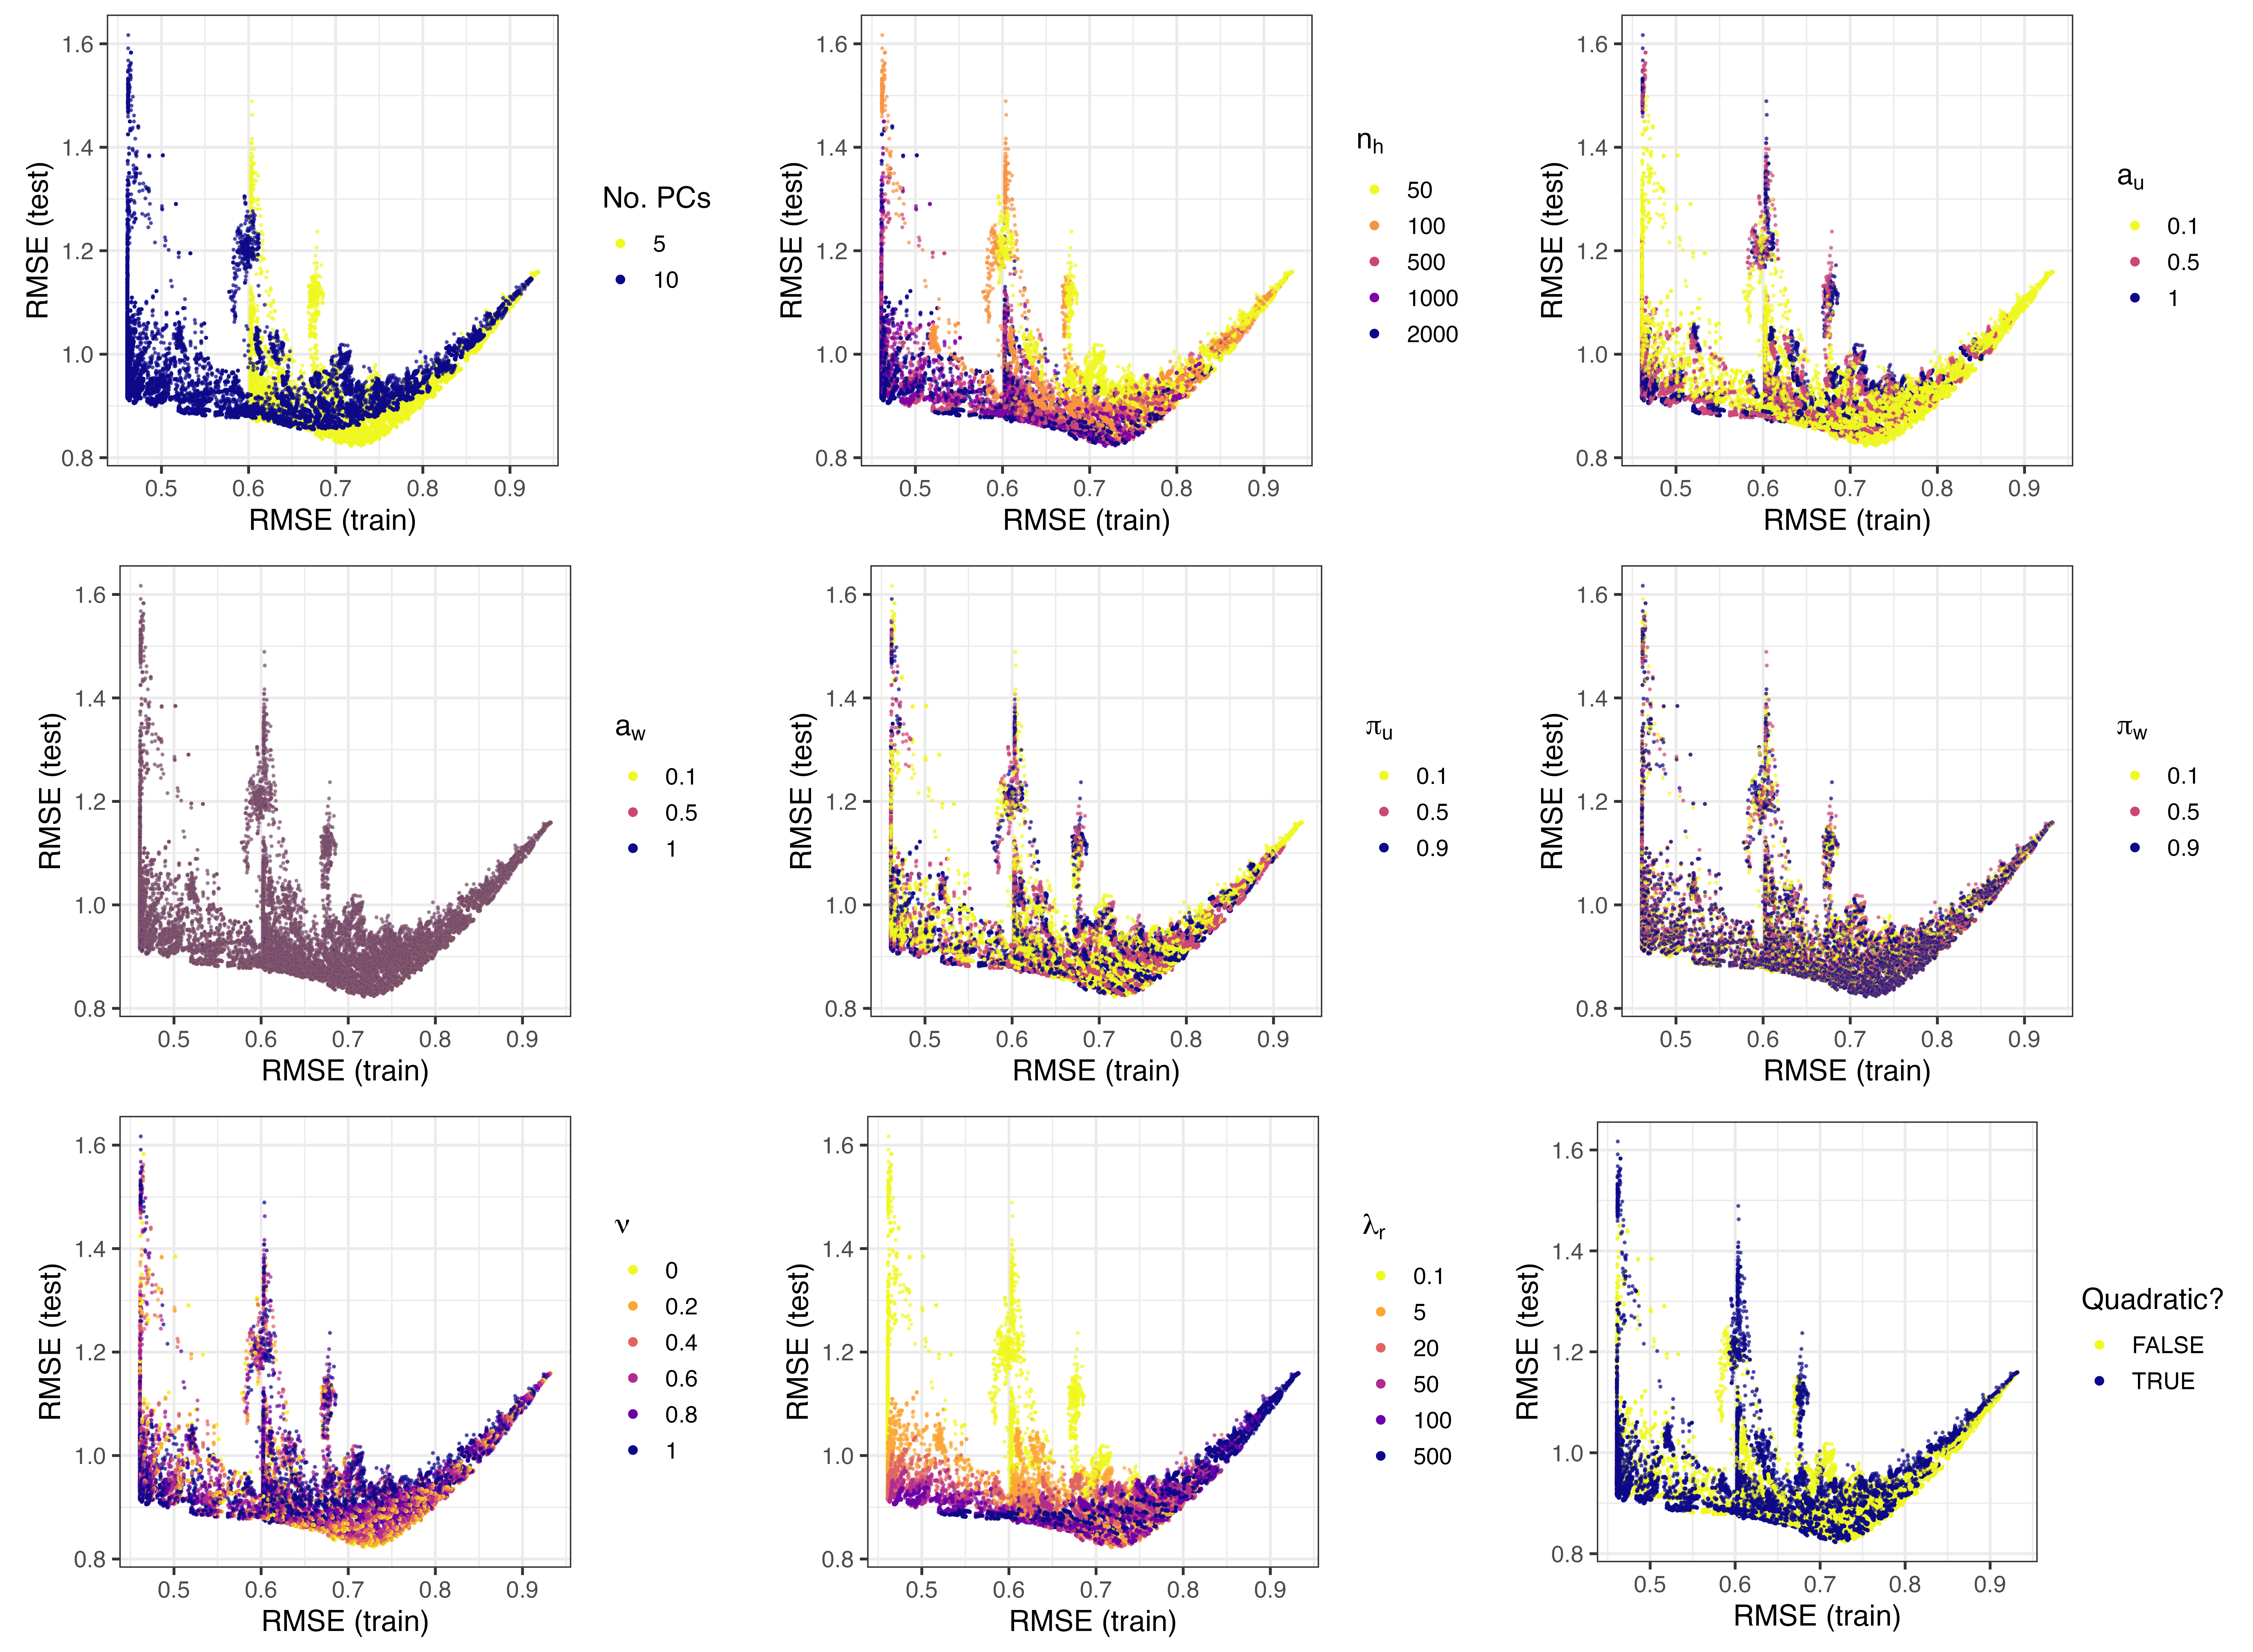
\includegraphics[width=\textwidth]{figures/merra2_hyper_param_all.png}
    \caption{Testing versus training weighted RMSEs from the MERRA-2 ESN hyperparameter search. Each plot is colored by the values considered for one of the hyperparameters.}
    \label{fig:hp_all}
\end{figure*}

\begin{figure*}[h]
    \centering
    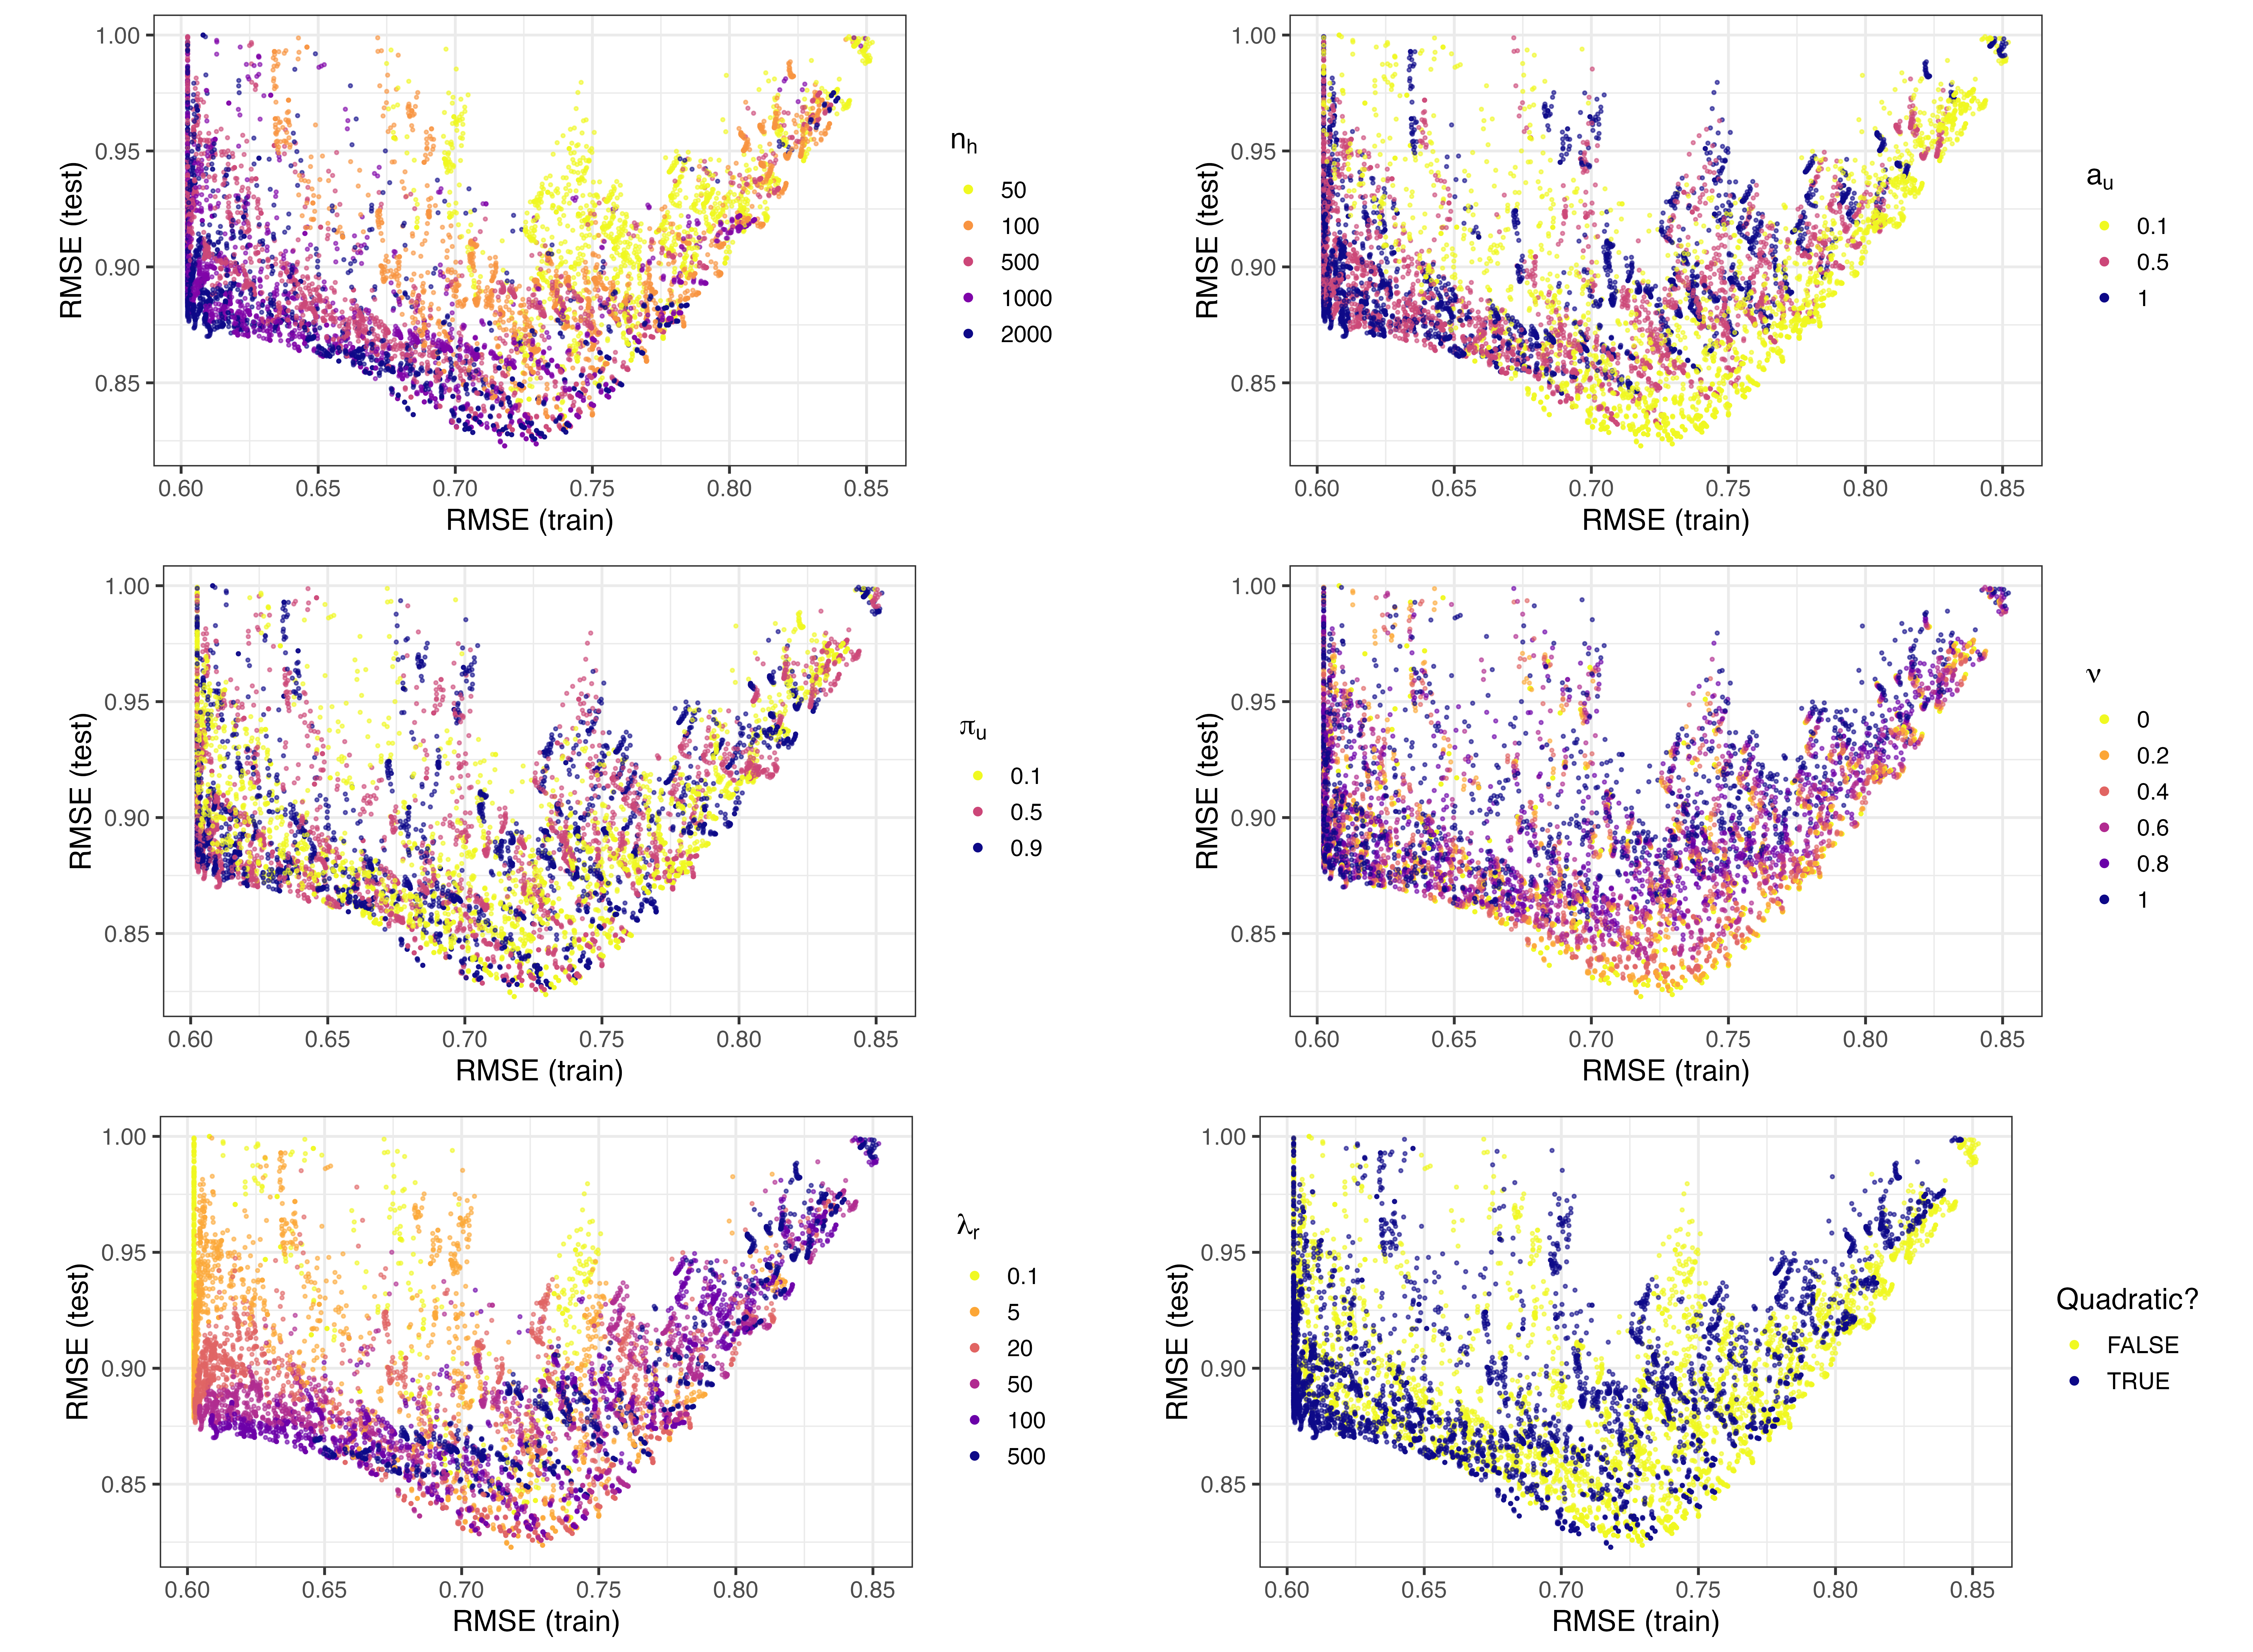
\includegraphics[width=\textwidth]{figures/merra2_hyper_param_sub.png}
    \caption{Testing versus training weighted RMSEs from the MERRA-2 ESN hyperparameter search subset to only contain test RMSEs less than 1, results from models trained with 5 principal components, and hyperparameters that have a clear effect on test RMSE.}
    \label{fig:hp_sub}
\end{figure*}

\begin{figure*}[h]
    \centering
    \includegraphics[width=\textwidth]{figures/merra2_hyper_param_uwidth.png}
    \caption{Violin plots of test RMSEs by $a_w$. Plots are separated by $n_h$, and points are colored by $\lambda_r$. Only RMSEs from ESNs fit with 5 principal components are included.}
    \label{fig:hp_uwidth}
    \vspace{1cm}
    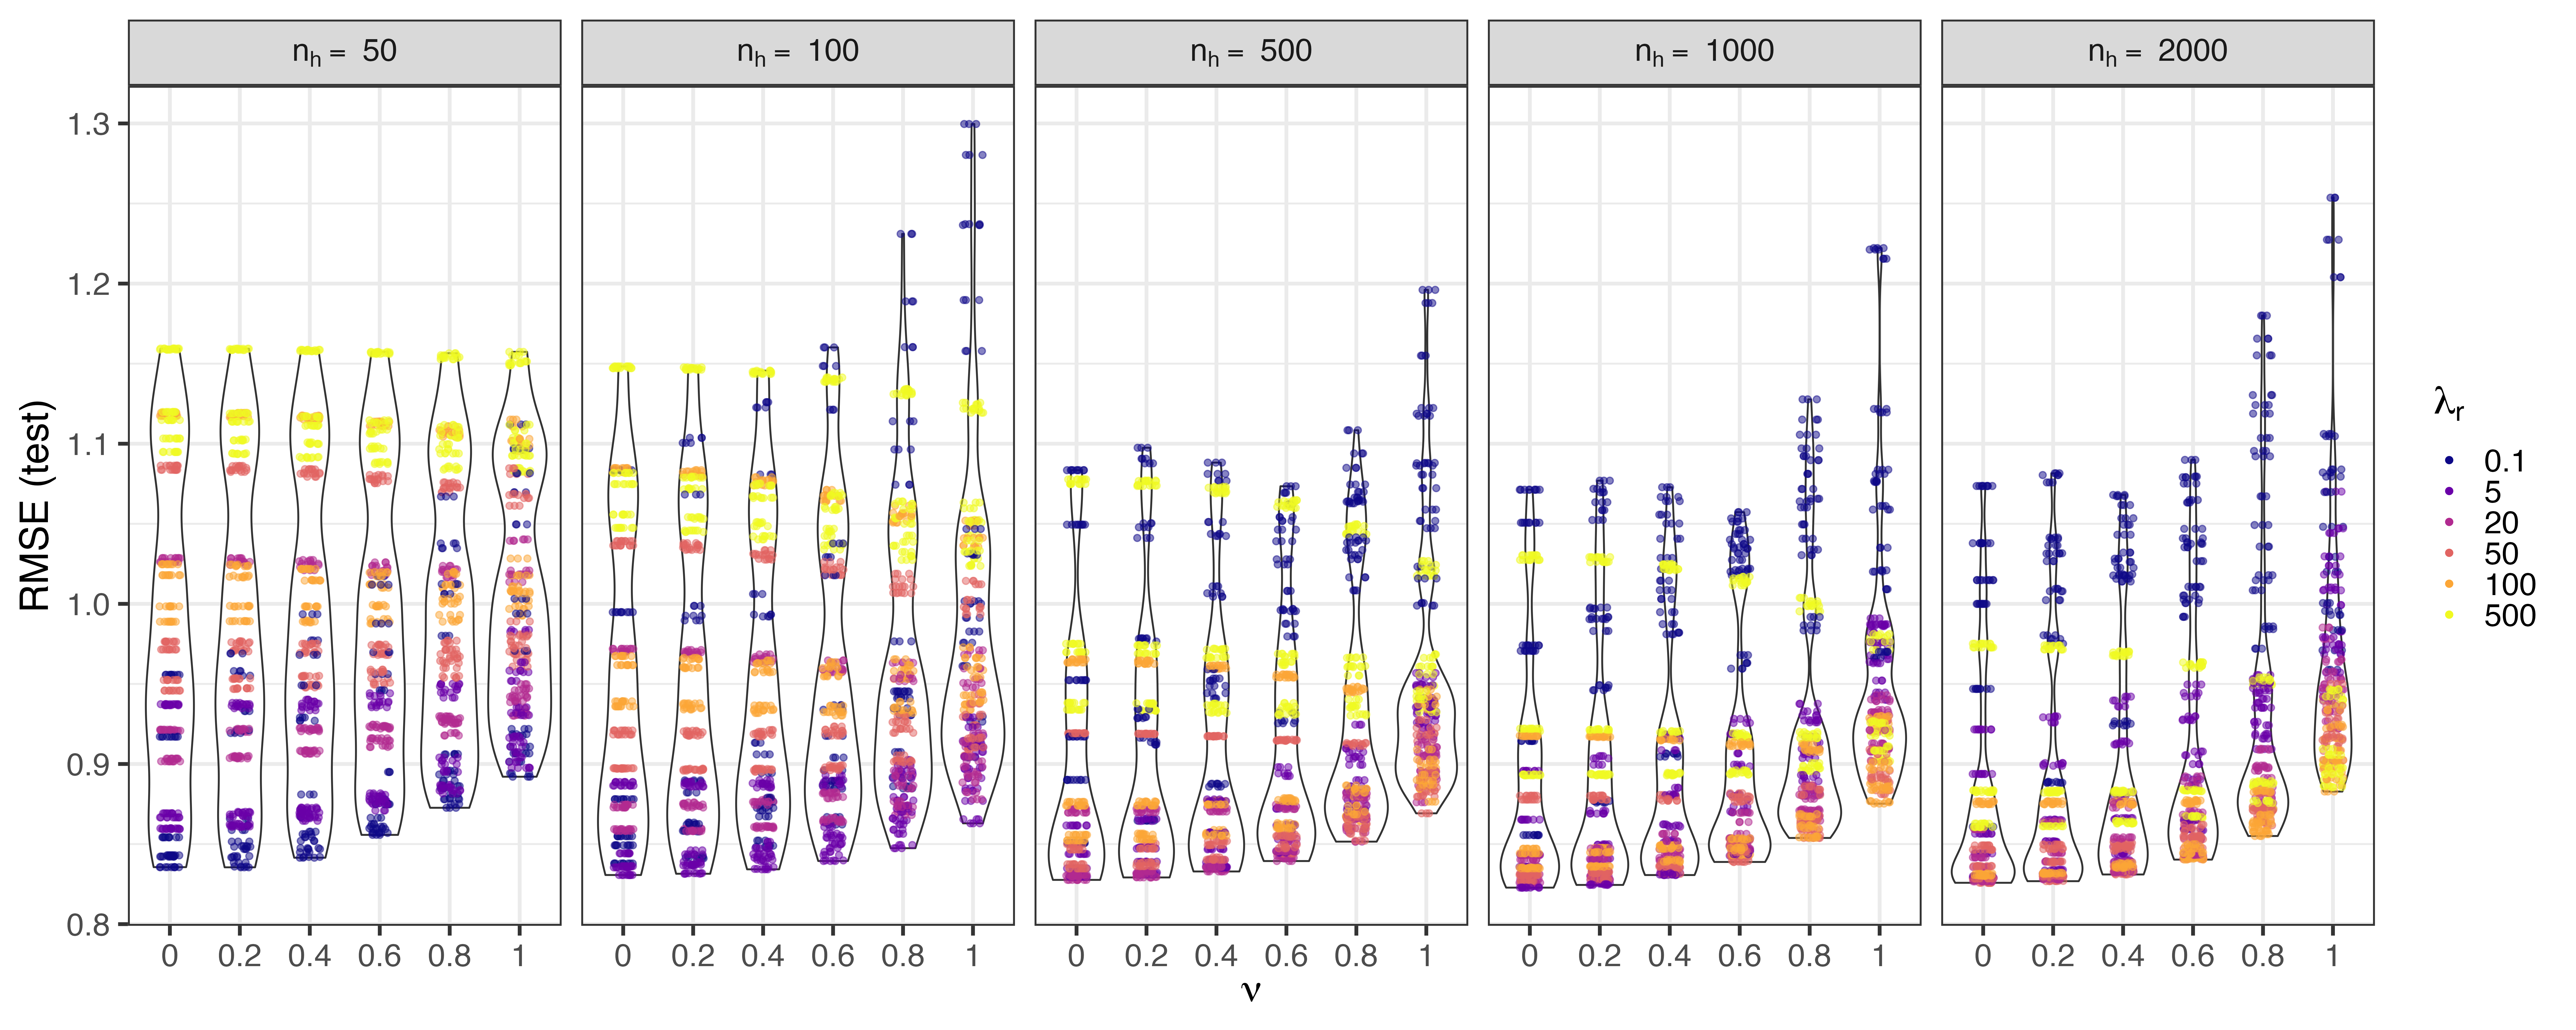
\includegraphics[width=\textwidth]{figures/merra2_hyper_param_nu.png}
    \caption{Violin plots of test RMSEs by $\nu$. Plots are separated by $n_h$, and points are colored by $\lambda_r$. Only RMSEs from ESNs fit with 5 principal components and $a_w=0.1$ are included.}
    \label{fig:hp_nu}
\end{figure*}

\begin{figure*}[h]
    \centering
    \includegraphics[width=\textwidth]{figures/merra2_hyper_param_nh_quad.png}
    \caption{Violin plots of test RMSEs by $n_h$. Plots are separated by $\lambda_r$, and points are colored by whether a quadratic term is included in the ridge regression. Only RMSEs from ESNs fit with 5 principal components, $a_w=0.1$, and $\nu=0.2$ are included.}
    \label{fig:hp_nh_quad}
    \vspace{1cm}
    \includegraphics[width=\textwidth]{figures/merra2_hyper_param_nh_upi.png}
    \caption{Violin plots of test RMSEs by $n_h$. Plots are separated by $\lambda_r$, and points are colored by $\pi_u$. Only RMSEs from ESNs fit with 5 principal components, $a_w=0.1$, and $\nu=0.2$ are included.}
    \label{fig:hp_nh_upi}
\end{figure*}

\begin{figure*}[h]
    \centering
    \includegraphics[width=\textwidth]{figures/merra2_rmse_anom.png}
    \caption{Weighted RMSEs on the normalized anomaly scale from the ESN blocked training/test splits on MERRA-2 data. Each row represents an additional one year of training data. Mount Pinatubo eruption is denoted by the vertical dashed line.}
    \label{fig:merra2rmseanom}
\end{figure*}

\begin{figure*}[h]
    \centering
    \includegraphics[width=\textwidth]{figures/merra2_rmse.png}
    \caption{Weighted RMSEs on the raw stratospheric temperature scale from the ESN blocked training/test splits on MERRA-2 data. Each row represents an additional one year of training data. Mount Pinatubo eruption is denoted by the vertical dashed line.}
    \label{fig:merra2rmse}
\end{figure*}

\begin{figure*}[h]
    \centering
    \includegraphics[width=0.9\textwidth]{figures/merra2_obs_pred.png}
    \caption{Example of observed vs predicted stratospheric temperatures (on raw stratospheric temperature scale) for ESN on MERRA-2 data for training and testing splits. The year in each row specifies through which year the model was trained on, with the remaining years through 1995 as test data. }
    \label{fig:merra2pred}
\end{figure*}

\begin{figure*}[h]
    \centering
    \includegraphics[width=\textwidth]{figures/merra2_fi_blocks_ens_aves.png}
    \caption{Feature importances for different block sizes on MERRA-2 averaged over the individual ESNs.}
    \label{fig:merra2blockave}
\end{figure*}

\begin{figure*}[h]
    \centering
    \includegraphics[width=\textwidth]{figures/merra2_fi_blocks_ens.png}
    \caption{Feature importances on MERRA-2 separated by block size to depict variability in FI across individual ESNs.}
    \label{fig:merra2block}
\end{figure*}

\begin{figure*}[h]
    \centering
    \includegraphics[width=\textwidth]{figures/merra2_fi_param_comparison.png}
    \caption{Feature importances from ESNs with different hyperparameters. The lines represent FIs computed with a block size of six and averaged over individual ESNs.}
    \label{fig:merra2fiparams}
\end{figure*}

\begin{figure*}[h]
    \centering
    \includegraphics[width=\textwidth]{figures/merra2_fi_param_var_comparison.png}
    \caption{Feature importances from ESNs with different hyperparameters. The lines represent FI computed with a block size of six for each of the individual ESNs.}
    \label{fig:merra2fiparamsvar}
\end{figure*}

\end{document}